% ============================================================================
% Results chapter
% Requires: graphicx, booktabs, amsmath, float
% ============================================================================

% Inserts the image if the file exists; otherwise shows a labelled placeholder.
% \detokenize prints the path literally, so underscores in filenames are safe.
\newcommand{\figslot}[1]{%
    \IfFileExists{#1}{%
        \includegraphics[width=\linewidth,height=0.45\textheight,keepaspectratio]{#1}%
    }{%
        \fbox{\parbox[c][0.3\textheight][c]{0.9\linewidth}{%
            \centering\texttt{[Missing: \detokenize{#1}]}}}%
    }%
}

% ============================================================================
\chapter{Results}
\label{chap:results}

This chapter reports the evolutionary optimization results for the suction-cup (SC) and
two-finger grippers. Bayesian optimization yielded some results, but these were limited in their usefulness. Each gripper--workpiece pair is
an independent optimization instance (Section~\ref{subsec:study_structure}), so
results are reported per workpiece and are not pooled across workpieces or
grippers.

The indicators are used as follows:
\begin{itemize}
    \item \textbf{Hypervolume (HV)} is compared across algorithms within a workpiece,
    because all runs share the same reference point.
    \item \textbf{IGD+} is computed against one shared reference front per workpiece. This
    front is built from the final solutions of all algorithms and runs on that workpiece.
    IGD+ is compared across algorithms within a workpiece, but not across workpieces.
    \item \textbf{Runtime} was measured on GPUs with different computing capacity. It is
    reported for information only and is not used for ranking.
\end{itemize}
All values are reported as mean $\pm$ sample standard deviation over independent runs.
In the tables, the best mean for IGD+ and HV is shown in bold.

% ============================================================================
\section{Suction-Cup Gripper Results}
\label{sec:results_sc}

\subsection{Preliminary Two-Objective Runs}
\label{subsec:results_sc_preliminary}

Initial test runs used two objectives, the normalized triangle area $\hat{A}$ and the
grasp diversity $D$. The resulting Pareto solutions contained only two grasps, mostly
located at opposite ends of the workpiece (Figure~\ref{fig:sc_preliminary_pareto}). Two
grasps at opposite ends already give a high diversity score, so maximizing $D$ favored
layouts with exactly two grasps and gave no incentive to retain additional distinct
grasps. For this reason, the normalized grasp count $\hat{n}_{\mathrm{g}}$ was added as a
third objective (Section~\ref{subsubsec:normalized_grasp_count}). All suction-cup results
below use this three-objective formulation.

\begin{figure}[H]
    \centering
    \figslot{fig/ch-result/SC_IPA_plate_2obj.png}
    \caption{Grasp points on the IPA Intermediate Plate from the two-objective
    suction-cup run (area and diversity).}
    \label{fig:sc_preliminary_pareto}
\end{figure}

\subsection{Experimental Settings}
\label{subsec:results_sc_settings}

Each evolutionary algorithm was run five times per workpiece, with a population of 100,
200 generations, and a budget of 20,000 evaluations (Table~\ref{tab:budget_termination}).
The archive HV is the best-so-far cumulative archive at termination. The reference point is
$-0.1$ in the natural maximization convention, which corresponds to $0.1$ in the
minimization convention used internally by the indicator.

\subsection{Individual Results per Workpiece}
\label{subsec:results_sc_individual}

\subsubsection{IPA Intermediate Plate}
\label{subsubsec:results_sc_ipa}

NSGA-II and SMS-EMOA form the leading group on this workpiece. SMS-EMOA gives the lowest
IGD+, and NSGA-II the highest archive HV, with SMS-EMOA nearly tied in HV. SMS-EMOA is the
only algorithm that combines the lowest IGD+ with an HV close to the best. CMOPSO and
NSGA-III form a middle group in HV, and MOEA/D is the weakest on both indicators. The
leading algorithms show a small run-to-run spread, whereas the IGD+ of MOEA/D varies more
between runs (Table~\ref{tab:sc_evo_intermediate_plate}).

\begin{table}[htbp]
    \centering
    \caption{Suction-cup results: IPA Intermediate Plate.}
    \label{tab:sc_evo_intermediate_plate}
    \begin{tabular}{@{}lccc@{}}
        \toprule
        \textbf{Algorithm} & \textbf{IGD+} $\downarrow$ & \textbf{Archive HV} $\uparrow$ & \textbf{Runtime (s)} \\
        \midrule
        CMOPSO   & $0.0131 \pm 0.0007$ & $0.3626 \pm 0.0045$ & $102500.4 \pm 2099.4$ \\
        MOEA/D   & $0.0312 \pm 0.0053$ & $0.3515 \pm 0.0084$ & $104270.6 \pm 2469.3$ \\
        NSGA-II  & $0.0122 \pm 0.0018$ & {\boldmath$0.3668 \pm 0.0011$} & $71979.8 \pm 785.4$ \\
        NSGA-III & $0.0133 \pm 0.0012$ & $0.3604 \pm 0.0057$ & $144361.2 \pm 1115.4$ \\
        SMS-EMOA & {\boldmath$0.0067 \pm 0.0003$} & $0.3664 \pm 0.0012$ & $67575.8 \pm 751.0$ \\
        \bottomrule
    \end{tabular}
\end{table}

\subsubsection{Knob}
\label{subsubsec:results_sc_knob}

NSGA-III, NSGA-II, and SMS-EMOA form a leading group that is close on both indicators.
NSGA-III has the highest archive HV, while SMS-EMOA has the lowest IGD+ of the three, so no
single algorithm leads on both. CMOPSO is clearly behind this group in HV. MOEA/D is the
weakest on both indicators, with the highest IGD+ and the lowest HV
(Table~\ref{tab:sc_evo_knob}).

\begin{table}[htbp]
    \centering
    \caption{Suction-cup results: Knob.}
    \label{tab:sc_evo_knob}
    \begin{tabular}{@{}lccc@{}}
        \toprule
        \textbf{Algorithm} & \textbf{IGD+} $\downarrow$ & \textbf{Archive HV} $\uparrow$ & \textbf{Runtime (s)} \\
        \midrule
        CMOPSO   & $0.0084 \pm 0.0006$ & $0.1449 \pm 0.0018$ & $56569.3 \pm 2020.7$ \\
        MOEA/D   & $0.0364 \pm 0.0048$ & $0.1168 \pm 0.0158$ & $82003.1 \pm 3013.8$ \\
        NSGA-II  & $0.0054 \pm 0.0007$ & $0.1617 \pm 0.0075$ & $63562.2 \pm 587.6$ \\
        NSGA-III & $0.0055 \pm 0.0023$ & {\boldmath$0.1639 \pm 0.0022$} & $53231.9 \pm 549.2$ \\
        SMS-EMOA & {\boldmath$0.0052 \pm 0.0017$} & $0.1602 \pm 0.0072$ & $46486.4 \pm 1317.1$ \\
        \bottomrule
    \end{tabular}
\end{table}

\subsubsection{Connecting Rod}
\label{subsubsec:results_sc_connecting_rod}

SMS-EMOA gives the lowest IGD+ and MOEA/D the highest, with NSGA-III second-highest. The
archive HV does not separate the algorithms. All five algorithms overlap within their
run-to-run spread, and the spreads of CMOPSO and MOEA/D are the widest. On this workpiece,
the IGD+ ranking is therefore the only clear distinction between the algorithms
(Table~\ref{tab:sc_evo_connecting_rod}).

\begin{table}[htbp]
    \centering
    \caption{Suction-cup results: Connecting rod.}
    \label{tab:sc_evo_connecting_rod}
    \begin{tabular}{@{}lccc@{}}
        \toprule
        \textbf{Algorithm} & \textbf{IGD+} $\downarrow$ & \textbf{Archive HV} $\uparrow$ & \textbf{Runtime (s)} \\
        \midrule
        CMOPSO   & $0.0162 \pm 0.0020$ & $0.2233 \pm 0.0153$ & $44538.9 \pm 1172.3$ \\
        MOEA/D   & $0.0307 \pm 0.0038$ & $0.2212 \pm 0.0146$ & $56479.5 \pm 3251.1$ \\
        NSGA-II  & $0.0172 \pm 0.0011$ & {\boldmath$0.2243 \pm 0.0107$} & $59928.5 \pm 1524.4$ \\
        NSGA-III & $0.0224 \pm 0.0016$ & $0.2183 \pm 0.0105$ & $48552.1 \pm 507.5$ \\
        SMS-EMOA & {\boldmath$0.0096 \pm 0.0016$} & $0.2210 \pm 0.0093$ & $40901.3 \pm 458.9$ \\
        \bottomrule
    \end{tabular}
\end{table}

\subsubsection{Stanford Bunny}
\label{subsubsec:results_sc_bunny}

SMS-EMOA gives the lowest IGD+ and the highest archive HV on the Stanford Bunny, with NSGA-II
a close second on both. CMOPSO and MOEA/D have the widest IGD+ spreads, so their positions
are the least certain. NSGA-III lies between the leading pair and CMOPSO on both indicators,
and MOEA/D is the weakest on both (Table~\ref{tab:sc_evo_bunny}).

\begin{table}[htbp]
    \centering
    \caption{Suction-cup results: Stanford Bunny.}
    \label{tab:sc_evo_bunny}
    \begin{tabular}{@{}lccc@{}}
        \toprule
        \textbf{Algorithm} & \textbf{IGD+} $\downarrow$ & \textbf{Archive HV} $\uparrow$ & \textbf{Runtime (s)} \\
        \midrule
        CMOPSO   & $0.0108 \pm 0.0034$ & $0.1068 \pm 0.0021$ & $81632.1 \pm 439.4$ \\
        MOEA/D   & $0.0189 \pm 0.0035$ & $0.1005 \pm 0.0059$ & $91043.0 \pm 1149.3$ \\
        NSGA-II  & $0.0049 \pm 0.0010$ & $0.1128 \pm 0.0038$ & $58394.7 \pm 801.2$ \\
        NSGA-III & $0.0086 \pm 0.0019$ & $0.1114 \pm 0.0025$ & $113785.4 \pm 1261.1$ \\
        SMS-EMOA & {\boldmath$0.0029 \pm 0.0002$} & {\boldmath$0.1131 \pm 0.0039$} & $52652.8 \pm 776.8$ \\
        \bottomrule
    \end{tabular}
\end{table}

\subsection{Cross-Workpiece Summary}
\label{subsec:results_sc_summary}

Figures~\ref{fig:sc_summary_igdplus}, \ref{fig:sc_summary_hv}, and \ref{fig:sc_summary_runtime}
show the three indicators for all algorithms and workpieces. Boxes show the median and
interquartile range, red markers show the mean $\pm$ one sample standard deviation, and dots
show individual runs ($n=5$ per algorithm).

\begin{figure}[H]
    \centering
    \figslot{fig/ch-result/SC_COMPLETED_igd_plus.png}
    \caption{IGD+ per workpiece and algorithm ($n=5$ runs per algorithm; lower is better).
    Values use the shared reference front of each workpiece.}
    \label{fig:sc_summary_igdplus}
\end{figure}

Figure~\ref{fig:sc_summary_igdplus} shows that SMS-EMOA has the lowest mean IGD+ on all four
workpieces, and MOEA/D the highest on all four. SMS-EMOA is also the most concentrated on the
IPA Intermediate Plate and the Stanford Bunny, whereas on the Knob CMOPSO and NSGA-II have a
smaller run-to-run spread, and on the Connecting rod NSGA-II does. NSGA-II is also tightly
grouped on every workpiece. On the Knob, the mean IGD+ values of NSGA-II, NSGA-III, and
SMS-EMOA lie within one standard deviation of each other, so these three are not clearly
separated.
The wide CMOPSO box on the Stanford Bunny and the wide MOEA/D boxes on several workpieces show
that run-to-run variation is large for these two algorithms. The conclusion is that SMS-EMOA
achieves the lowest mean IGD+ for the suction cup on all four workpieces, although its
run-to-run spread is not the smallest on every workpiece, while MOEA/D is consistently the
weakest.

\begin{figure}[H]
    \centering
    \figslot{fig/ch-result/SC_COMPLETED_archive_hv_final.png}
    \caption{Final archive hypervolume per workpiece and algorithm ($n=5$ runs per algorithm;
    higher is better).}
    \label{fig:sc_summary_hv}
\end{figure}

Figure~\ref{fig:sc_summary_hv} shows that the boxes separate the algorithms on three of the
four workpieces. On the Stanford Bunny, the boxes of NSGA-II, NSGA-III, and SMS-EMOA form a
group that lies entirely above those of CMOPSO and MOEA/D. On the IPA Intermediate Plate, the
boxes of NSGA-II and SMS-EMOA are high and tight, and CMOPSO lies just below them without
overlap. NSGA-III has a wider box in the middle, and MOEA/D is lowest with the widest spread.
On the Knob, the boxes of NSGA-II, NSGA-III, and SMS-EMOA are high and overlap, CMOPSO lies
clearly below this group, and MOEA/D is lowest, with one run well above its box. On the
Connecting rod, by contrast, the boxes of all five algorithms overlap across nearly the same
range, and the means lie within about one standard deviation of each other, so no algorithm
is separated. The conclusion is that HV distinguishes the algorithms on the Stanford Bunny,
the IPA Intermediate Plate, and the Knob, where MOEA/D is lowest on each. On the Connecting
rod, HV does not distinguish them conclusively.

\begin{figure}[H]
    \centering
    \figslot{fig/ch-result/SC_COMPLETED_runtime_s.png}
    \caption{Wall-clock time per workpiece and algorithm ($n=5$ runs per algorithm; seconds;
    indicative only, as the runs used different GPUs).}
    \label{fig:sc_summary_runtime}
\end{figure}

Figure~\ref{fig:sc_summary_runtime} shows that run-to-run spread is small for most
algorithm--workpiece combinations. The ordering of the algorithms changes between workpieces.
For example, NSGA-III is the slowest on the Stanford Bunny and the IPA Intermediate Plate,
while NSGA-II is the slowest on the Connecting rod and MOEA/D on the Knob. Because the runs used
different GPUs, these differences cannot be separated from hardware effects. The figure is
therefore used only to describe the computational cost, and no runtime ranking is drawn.

\subsection{Hypervolume Progression}
\label{subsec:results_sc_progression}

\begin{figure}[H]
    \centering
    \figslot{fig/ch-result/SC_COMPLETED_hv_progression.png}
    \caption{Cumulative archive hypervolume over evaluations, per workpiece and algorithm
    (mean across $n=5$ runs; shading: $\pm 1$ sample SD).}
    \label{fig:sc_hv_progression}
\end{figure}

Figure~\ref{fig:sc_hv_progression} shows that most curves rise steeply in the first part of
the run and then flatten gradually. Several curves are still rising at the end of the budget,
particularly on the Stanford Bunny and the IPA Intermediate Plate. The final HV values
therefore reflect the 20,000-evaluation budget as well as the algorithm quality.

On the Stanford Bunny, MOEA/D is briefly ahead at the start, but it falls behind early and
then stays at the lowest level, with little change after the middle of the run. SMS-EMOA and
NSGA-II lead for most of the run, with NSGA-III and CMOPSO following. On the Connecting rod,
MOEA/D leads during the early phase, but the other algorithms overtake it, and all curves merge
into a narrow band from about the middle of the run. CMOPSO shows a late step in the final part
of the run. On the IPA Intermediate Plate, the curves stay close together throughout. MOEA/D is
consistently lowest, and SMS-EMOA and NSGA-II are highest at the end while still rising. On the
Knob, NSGA-II, NSGA-III, and SMS-EMOA rise together within a narrow band, and NSGA-III is still
increasing at the end. CMOPSO reaches a plateau earlier at a lower level. MOEA/D rises slowly,
shows a step in the middle of the run, and has a very wide band, which indicates that its runs
diverge.

The conclusion is that the final ranking of the algorithms is mostly determined in the second
half of the run. The early lead of MOEA/D on the Stanford Bunny and the Connecting rod does not
persist.

% ============================================================================
\section{Two-Finger Gripper Results}
\label{sec:results_tf}

\subsection{Experimental Settings}
\label{subsec:results_tf_settings}

Each evolutionary algorithm was run three times per workpiece, with a population of 100,
100 generations, and a budget of 10,000 evaluations. The problem has four objectives, one
grasp-quality KPI per predefined grasp orientation. The archive HV and the reference point are
defined as for the suction-cup gripper. The IGD+ reference front of each workpiece is pooled from
the final solutions of all five algorithms and three runs (15 runs) on that workpiece.

\subsection{Individual Results per Workpiece}
\label{subsec:results_tf_individual}

\subsubsection{IPA Intermediate Plate}
\label{subsubsec:results_tf_ipa}

NSGA-II has the highest archive HV, closely followed by SMS-EMOA. SMS-EMOA gives the lowest
IGD+, with NSGA-II within the run-to-run spread. CMOPSO and MOEA/D lie lower in HV, and MOEA/D
is the weakest on both indicators, with the highest IGD+. NSGA-III has the widest HV spread on
this workpiece (Table~\ref{tab:tf_evo_intermediate_plate}).

\begin{table}[htbp]
    \centering
    \caption{Two-finger results: IPA Intermediate Plate.}
    \label{tab:tf_evo_intermediate_plate}
    \begin{tabular}{@{}lccc@{}}
        \toprule
        \textbf{Algorithm} & \textbf{IGD+} $\downarrow$ & \textbf{Archive HV} $\uparrow$ & \textbf{Runtime (s)} \\
        \midrule
        CMOPSO   & $0.0310 \pm 0.0094$ & $0.0915 \pm 0.0038$ & $25014.9 \pm 7.1$ \\
        MOEA/D   & $0.0438 \pm 0.0155$ & $0.0851 \pm 0.0061$ & $66839.0 \pm 20.3$ \\
        NSGA-II  & $0.0148 \pm 0.0020$ & {\boldmath$0.1138 \pm 0.0010$} & $41697.5 \pm 12602.0$ \\
        NSGA-III & $0.0233 \pm 0.0077$ & $0.1082 \pm 0.0120$ & $37865.6 \pm 25243.9$ \\
        SMS-EMOA & {\boldmath$0.0140 \pm 0.0044$} & $0.1110 \pm 0.0071$ & $67543.7 \pm 11.6$ \\
        \bottomrule
    \end{tabular}
\end{table}

\subsubsection{Knob}
\label{subsubsec:results_tf_knob}

NSGA-II has the highest archive HV and the lowest IGD+, with CMOPSO close on IGD+. SMS-EMOA is
second on HV but sits in the middle on IGD+. NSGA-III has the highest IGD+. MOEA/D has the
lowest HV, clearly separated from the other four algorithms, which lie close together
(Table~\ref{tab:tf_evo_knob}).

\begin{table}[htbp]
    \centering
    \caption{Two-finger results: Knob.}
    \label{tab:tf_evo_knob}
    \begin{tabular}{@{}lccc@{}}
        \toprule
        \textbf{Algorithm} & \textbf{IGD+} $\downarrow$ & \textbf{Archive HV} $\uparrow$ & \textbf{Runtime (s)} \\
        \midrule
        CMOPSO   & $0.0050 \pm 0.0014$ & $1.3491 \pm 0.0072$ & $27087.4 \pm 1.2$ \\
        MOEA/D   & $0.0075 \pm 0.0004$ & $1.3268 \pm 0.0057$ & $24614.5 \pm 211.5$ \\
        NSGA-II  & {\boldmath$0.0049 \pm 0.0005$} & {\boldmath$1.3572 \pm 0.0083$} & $46510.5 \pm 13589.5$ \\
        NSGA-III & $0.0084 \pm 0.0014$ & $1.3461 \pm 0.0065$ & $38328.5 \pm 24973.1$ \\
        SMS-EMOA & $0.0062 \pm 0.0016$ & $1.3550 \pm 0.0098$ & $75822.1 \pm 13.0$ \\
        \bottomrule
    \end{tabular}
\end{table}

\subsubsection{Connecting Rod}
\label{subsubsec:results_tf_connecting_rod}

NSGA-II is best on both indicators, with CMOPSO close on IGD+ and SMS-EMOA close on HV. The
top three algorithms in HV differ little. NSGA-III has the second-highest IGD+. MOEA/D is
clearly the weakest on both indicators (Table~\ref{tab:tf_evo_connecting_rod}).

\begin{table}[htbp]
    \centering
    \caption{Two-finger results: Connecting rod.}
    \label{tab:tf_evo_connecting_rod}
    \begin{tabular}{@{}lccc@{}}
        \toprule
        \textbf{Algorithm} & \textbf{IGD+} $\downarrow$ & \textbf{Archive HV} $\uparrow$ & \textbf{Runtime (s)} \\
        \midrule
        CMOPSO   & $0.0141 \pm 0.0007$ & $0.0309 \pm 0.0003$ & $27849.4 \pm 1.7$ \\
        MOEA/D   & $0.0281 \pm 0.0033$ & $0.0259 \pm 0.0003$ & $72605.3 \pm 14.3$ \\
        NSGA-II  & {\boldmath$0.0138 \pm 0.0009$} & {\boldmath$0.0323 \pm 0.0003$} & $46526.8 \pm 14061.9$ \\
        NSGA-III & $0.0198 \pm 0.0023$ & $0.0318 \pm 0.0008$ & $38407.6 \pm 24954.0$ \\
        SMS-EMOA & $0.0151 \pm 0.0020$ & $0.0320 \pm 0.0003$ & $30505.6 \pm 7.9$ \\
        \bottomrule
    \end{tabular}
\end{table}

\subsubsection{Stanford Bunny}
\label{subsubsec:results_tf_bunny}

SMS-EMOA gives the lowest IGD+ and NSGA-II the highest archive HV. Neither algorithm dominates
the other across both indicators, since SMS-EMOA lies within the HV spread of NSGA-II. CMOPSO
and NSGA-III lie in the middle, with the IGD+ of NSGA-III clearly higher. MOEA/D is the weakest
on both indicators, with a much lower HV than all other algorithms
(Table~\ref{tab:tf_evo_bunny}).

\begin{table}[htbp]
    \centering
    \caption{Two-finger results: Stanford Bunny.}
    \label{tab:tf_evo_bunny}
    \begin{tabular}{@{}lccc@{}}
        \toprule
        \textbf{Algorithm} & \textbf{IGD+} $\downarrow$ & \textbf{Archive HV} $\uparrow$ & \textbf{Runtime (s)} \\
        \midrule
        CMOPSO   & $0.0300 \pm 0.0031$ & $0.5937 \pm 0.0009$ & $25498.5 \pm 3.0$ \\
        MOEA/D   & $0.0529 \pm 0.0053$ & $0.5406 \pm 0.0058$ & $24111.3 \pm 113.4$ \\
        NSGA-II  & $0.0296 \pm 0.0041$ & {\boldmath$0.5999 \pm 0.0078$} & $43799.9 \pm 13306.3$ \\
        NSGA-III & $0.0410 \pm 0.0024$ & $0.5955 \pm 0.0041$ & $38078.9 \pm 25104.9$ \\
        SMS-EMOA & {\boldmath$0.0248 \pm 0.0024$} & $0.5997 \pm 0.0067$ & $27821.6 \pm 0.7$ \\
        \bottomrule
    \end{tabular}
\end{table}

\subsection{Cross-Workpiece Summary}
\label{subsec:results_tf_summary}

Figures~\ref{fig:tf_summary_igdplus}, \ref{fig:tf_summary_hv}, and \ref{fig:tf_summary_runtime}
show the three indicators for all algorithms and workpieces. Boxes show the median and
interquartile range, red markers show the mean $\pm$ one sample standard deviation, and dots
show individual runs ($n=3$ per algorithm).

\begin{figure}[H]
    \centering
    \figslot{fig/ch-result/PJ_COMPLETED_igd_plus.png}
    \caption{IGD+ per workpiece and algorithm ($n=3$ runs per algorithm; lower is better).
    Values use the shared reference front of each workpiece.}
    \label{fig:tf_summary_igdplus}
\end{figure}

Figure~\ref{fig:tf_summary_igdplus} shows that MOEA/D has the highest IGD+ on the Stanford
Bunny, the Connecting rod, and the IPA Intermediate Plate, with its box clearly above the
others on the first two. On the Knob, NSGA-III has the highest IGD+, and MOEA/D lies above
the lower group formed by CMOPSO and NSGA-II, whose boxes overlap. On the Connecting rod,
CMOPSO and NSGA-II form the lowest group, with their boxes overlapping. On the IPA
Intermediate Plate, the NSGA-II and SMS-EMOA boxes form the lowest group, while the CMOPSO
and MOEA/D boxes are wide and only partly separated from them. SMS-EMOA is lowest on the
Stanford Bunny. The conclusion is that no algorithm is lowest on all four workpieces. MOEA/D
is the highest on three of the four and lies in the upper group on the fourth, while NSGA-II
is in the lowest group on three of the four.

\begin{figure}[H]
    \centering
    \figslot{fig/ch-result/PJ_COMPLETED_archive_hv_final.png}
    \caption{Final archive hypervolume per workpiece and algorithm ($n=3$ runs per algorithm;
    higher is better).}
    \label{fig:tf_summary_hv}
\end{figure}

Figure~\ref{fig:tf_summary_hv} shows that NSGA-II is highest or tied for highest on every
workpiece, and MOEA/D is lowest on every workpiece, separated from the other algorithms on the
Bunny and the Connecting rod. On the Connecting rod, NSGA-II, SMS-EMOA, and NSGA-III are close
and tight. On the IPA Intermediate Plate, NSGA-II is tight and highest, while NSGA-III and SMS-EMOA
have wide boxes that overlap with the middle group. On the Knob, SMS-EMOA has a wide box close to
NSGA-II. The conclusion is that NSGA-II achieved the highest mean HV within each workpiece, and MOEA/D the least.

\begin{figure}[H]
    \centering
    \figslot{fig/ch-result/PJ_COMPLETED_runtime_s.png}
    \caption{Wall-clock time per workpiece and algorithm ($n=3$ runs per algorithm; seconds;
    indicative only, as the runs used different GPUs).}
    \label{fig:tf_summary_runtime}
\end{figure}

Figure~\ref{fig:tf_summary_runtime} shows that CMOPSO and SMS-EMOA have narrow runtime spreads.
NSGA-II and NSGA-III show a split pattern on each workpiece. Most of their runs are long, while
one run is much shorter. The short runs are most likely caused by hardware differences, as stated
above, but this cannot be verified from the data. MOEA/D is among the slowest on the Connecting
rod and the IPA Intermediate Plate, and among the fastest on the Stanford Bunny and the Knob. The
conclusion is that the runtime pattern is not interpretable as an algorithm property, and no
runtime ranking is drawn.

\subsection{Hypervolume Progression}
\label{subsec:results_tf_progression}

\begin{figure}[H]
    \centering
    \figslot{fig/ch-result/PJ_COMPLETED_hv_progression.png}
    \caption{Cumulative archive hypervolume over evaluations, per workpiece and algorithm
    (mean across $n=3$ runs; shading: $\pm 1$ sample SD).}
    \label{fig:tf_hv_progression}
\end{figure}

Figure~\ref{fig:tf_hv_progression} shows that the Knob converges fastest. All algorithms reach a
close, flat final level after the early part of the run, with narrow bands. MOEA/D rises fastest
at the start on the Knob, but the other algorithms catch up and MOEA/D ends lowest, so its early
advantage is not kept.

On the Stanford Bunny, MOEA/D rises quickly in the early phase, but it flattens at the lowest level
at around the first fifth of the run. The other four algorithms overlap and keep rising slowly
until the end, converging to a narrow band from the middle of the run. On the Connecting rod,
MOEA/D grows slowly and stays far below the others. The other four rise steeply early and keep
improving until the end. NSGA-II ends highest and is still rising. On the IPA Intermediate Plate,
the trajectories differ most. CMOPSO and MOEA/D flatten early, with CMOPSO stagnating from the
middle of the run. NSGA-II keeps rising until the end and ends highest. NSGA-III and SMS-EMOA are
also still rising at the end, with wide bands.

The conclusion is that for the Knob, the hypervolume curves plateaued within the
available budget, the Connecting rod and the Stanford Bunny are close to
convergence, and the IPA Intermediate Plate is not converged for NSGA-II,
NSGA-III, and SMS-EMOA at 10,000 evaluations. The early speed of MOEA/D does not
translate into the
final HV on any workpiece.

% ============================================================================
\section{Qualitative Inspection of Selected Solutions}
\label{sec:qualitative_inspection}

This section complements the quantitative results with a visual
inspection of selected Pareto solutions. One solution is shown for
each gripper--workpiece combination. For each instance, a run among
the best or second-best runs across the compared algorithms was
selected using either final archive hypervolume or IGD+. A solution
from that run was then selected manually to favor high values across
the objectives. This selection represents a subjective compromise
rather than the result of a formal decision-making criterion.

The examples illustrate individual trade-offs and are not necessarily
representative of the complete Pareto fronts. Since the images are
generated using the same evaluation pipelines as the optimization,
they do not independently validate those pipelines or establish
physical grasp feasibility.

The objective values below are reported in the natural maximization
convention. Values stored by the evolutionary framework were negated
for minimization and have therefore been negated again for presentation.
Decision variables and objective values are rounded.

\subsection{Qualitative Inspection of Multi-Suction Cup Gripper}
\label{subsec:qualitative_suction}

Figure~\ref{fig:qualitative_suction} shows the retained grasp sets for
four selected suction-cup layouts. Green square markers indicate the suction-cup
positions, yellow markers indicate the tool center point (TCP), and the red,
green, and blue lines indicate the axes of the grasp pose. The translucent
triangles connect the three cup positions at each grasp pose. The figures show
the grasp sets used to calculate diversity and normalized grasp count explained
in Section~\ref{sec:multi_sc_objective_evaluation}.

\begin{figure}[H]
    \centering
    \begin{subfigure}[t]{0.48\textwidth}
        \centering
        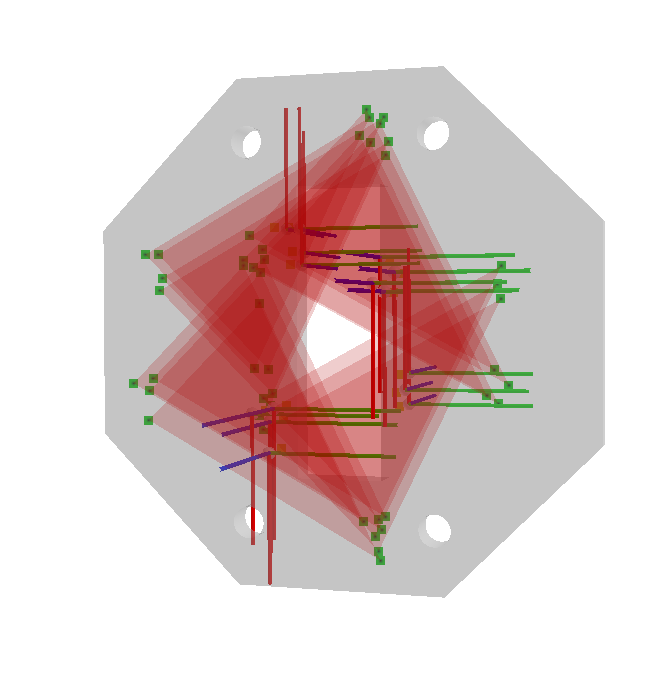
\includegraphics[
            width=\linewidth,
            height=0.23\textheight,
            keepaspectratio
        ]{fig/ch-validation/suctioncup_IPAIntermediatePlate_SMSEMOA_200Gen.png}
        \caption{IPA Intermediate Plate; SMS-EMOA}
        \label{fig:qualitative_sc_plate}
    \end{subfigure}\hfill
    \begin{subfigure}[t]{0.48\textwidth}
        \centering
        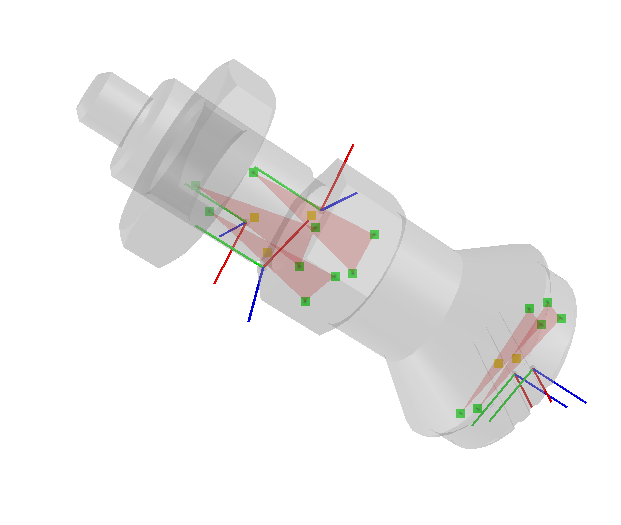
\includegraphics[
            width=\linewidth,
            height=0.23\textheight,
            keepaspectratio
        ]{fig/ch-validation/suctioncup_MCBA_Knob_NSGA3_200Gen.png}
        \caption{Knob; NSGA-III}
        \label{fig:qualitative_sc_knob}
    \end{subfigure}

    \par\medskip

    \begin{subfigure}[t]{0.48\textwidth}
        \centering
        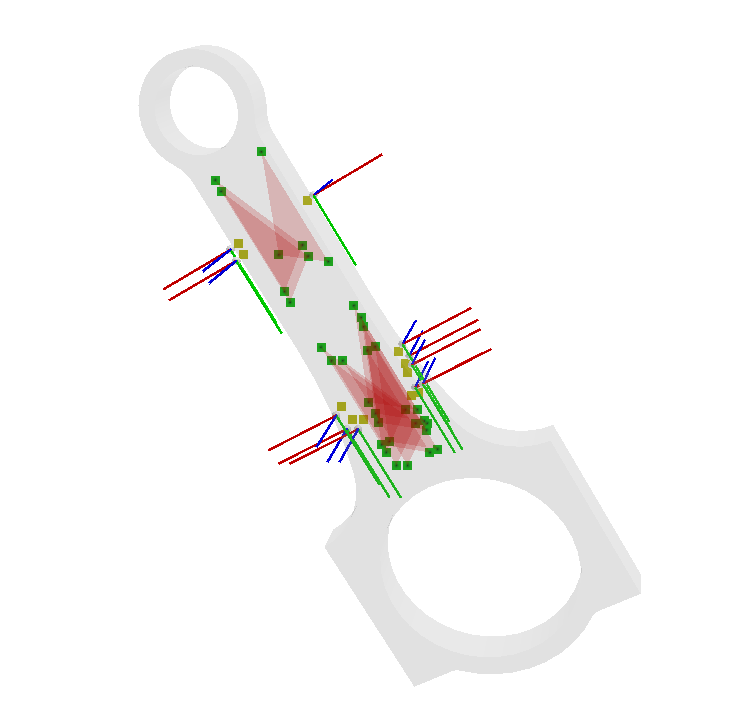
\includegraphics[
            width=\linewidth,
            height=0.23\textheight,
            keepaspectratio
        ]{fig/ch-validation/suctioncup_IPAConnectingRod_SMSEMOA_200Gen.png}
        \caption{Connecting rod; SMS-EMOA}
        \label{fig:qualitative_sc_rod}
    \end{subfigure}\hfill
    \begin{subfigure}[t]{0.48\textwidth}
        \centering
        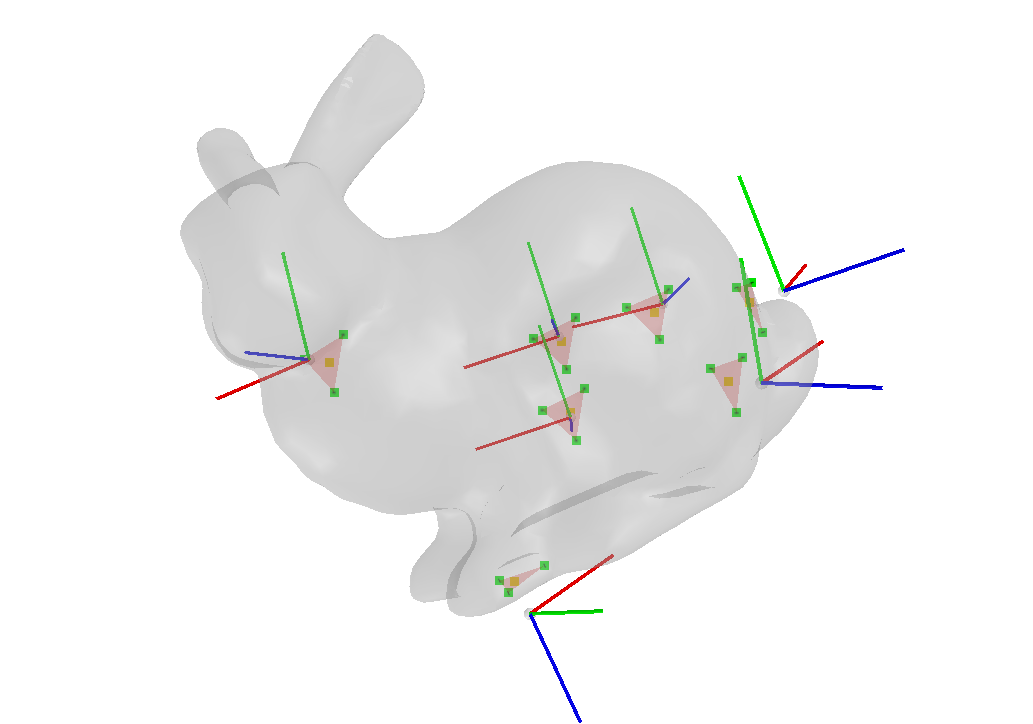
\includegraphics[
            width=\linewidth,
            height=0.23\textheight,
            keepaspectratio
        ]{fig/ch-validation/suctioncup_IPABunny_SMSEMOA_200Gen.png}
        \caption{Stanford Bunny; SMS-EMOA}
        \label{fig:qualitative_sc_bunny}
    \end{subfigure}

    \caption{Retained grasp sets for selected multi-suction-cup
    solutions. Each translucent triangle connects the three cup
    positions at one grasp pose.}
    \label{fig:qualitative_suction}
\end{figure}

For each layout, the decision vector is
$\mathbf{q}_{\mathrm{SC}}=(r,\alpha_1,\alpha_2,\alpha_3)$, where
$r$ is in meters and the angles are in radians. The objective vector
is $(D,\hat{n}_{\mathrm{g}},\hat{A})$:

\begin{itemize}
    \item \textbf{IPA Intermediate Plate:}
    $\mathbf{q}_{\mathrm{SC}}\approx
    (0.023124,\,3.2962,\,0.7594,\,4.5371)$;
    objectives $(0.4193,\,1.0000,\,0.1965)$;
    15 retained grasps.

    \item \textbf{Knob:}
    $\mathbf{q}_{\mathrm{SC}}\approx
    (0.018171,\,1.5032,\,4.3042,\,4.9955)$;
    objectives $(0.5252,\,0.3333,\,0.0757)$;
    5 retained grasps.

    \item \textbf{Connecting rod:}
    $\mathbf{q}_{\mathrm{SC}}\approx
    (0.015658,\,2.6149,\,1.7993,\,4.4834)$;
    objectives $(0.4704,\,0.7333,\,0.0531)$;
    11 retained grasps.

    \item \textbf{Stanford Bunny:}
    $\mathbf{q}_{\mathrm{SC}}\approx
    (0.005529,\,2.4223,\,0.4289,\,4.8284)$;
    objectives $(0.4419,\,0.4667,\,0.0135)$;
    7 retained grasps.
\end{itemize}

The grasp counts correspond to the normalized grasp-count objective
with $K_{\mathrm{clst}}=15$. The figures show grasps in different
regions of each workpiece. Some grasps are concentrated in particular
areas, as visible on the connecting rod, while the plate and Bunny
examples show grasps across multiple surface regions.

The positions and pose axes provide an intuitive impression of spatial
and orientational diversity. However, the diversity objective combines
normalized pairwise measures, so its numerical value cannot be
determined from the images alone. Similarly, the triangles illustrate
the cup arrangement, but their apparent size depends on the viewing
projection.

The figures illustrate the grasp sets produced by the computational
evaluation. They do not establish that the layouts will form seals or
withstand external loads in a physical grasp.

\subsection{Qualitative Inspection of Two-Finger Gripper}
\label{subsec:qualitative_two_finger}

Figure~\ref{fig:qualitative_two_finger} shows combined occupancy
projections for the selected parallel-jaw solutions. For each
workpiece, the displayed image corresponds to the predefined
orientation with the highest proximity KPI for that solution.

As described in
Section~\ref{subsec:objective_two_finger_gripper}, the workpiece
voxel grid is shifted using the selected left-jaw index and combined
with the gripper grid in its modeled pose. The image is
obtained by summing occupied voxels along the gripper length axis and its
colors therefore represent projected occupancy rather than proximity
scores.

\begin{figure}[H]
    \centering
    \begin{subfigure}[t]{0.48\textwidth}
        \centering
        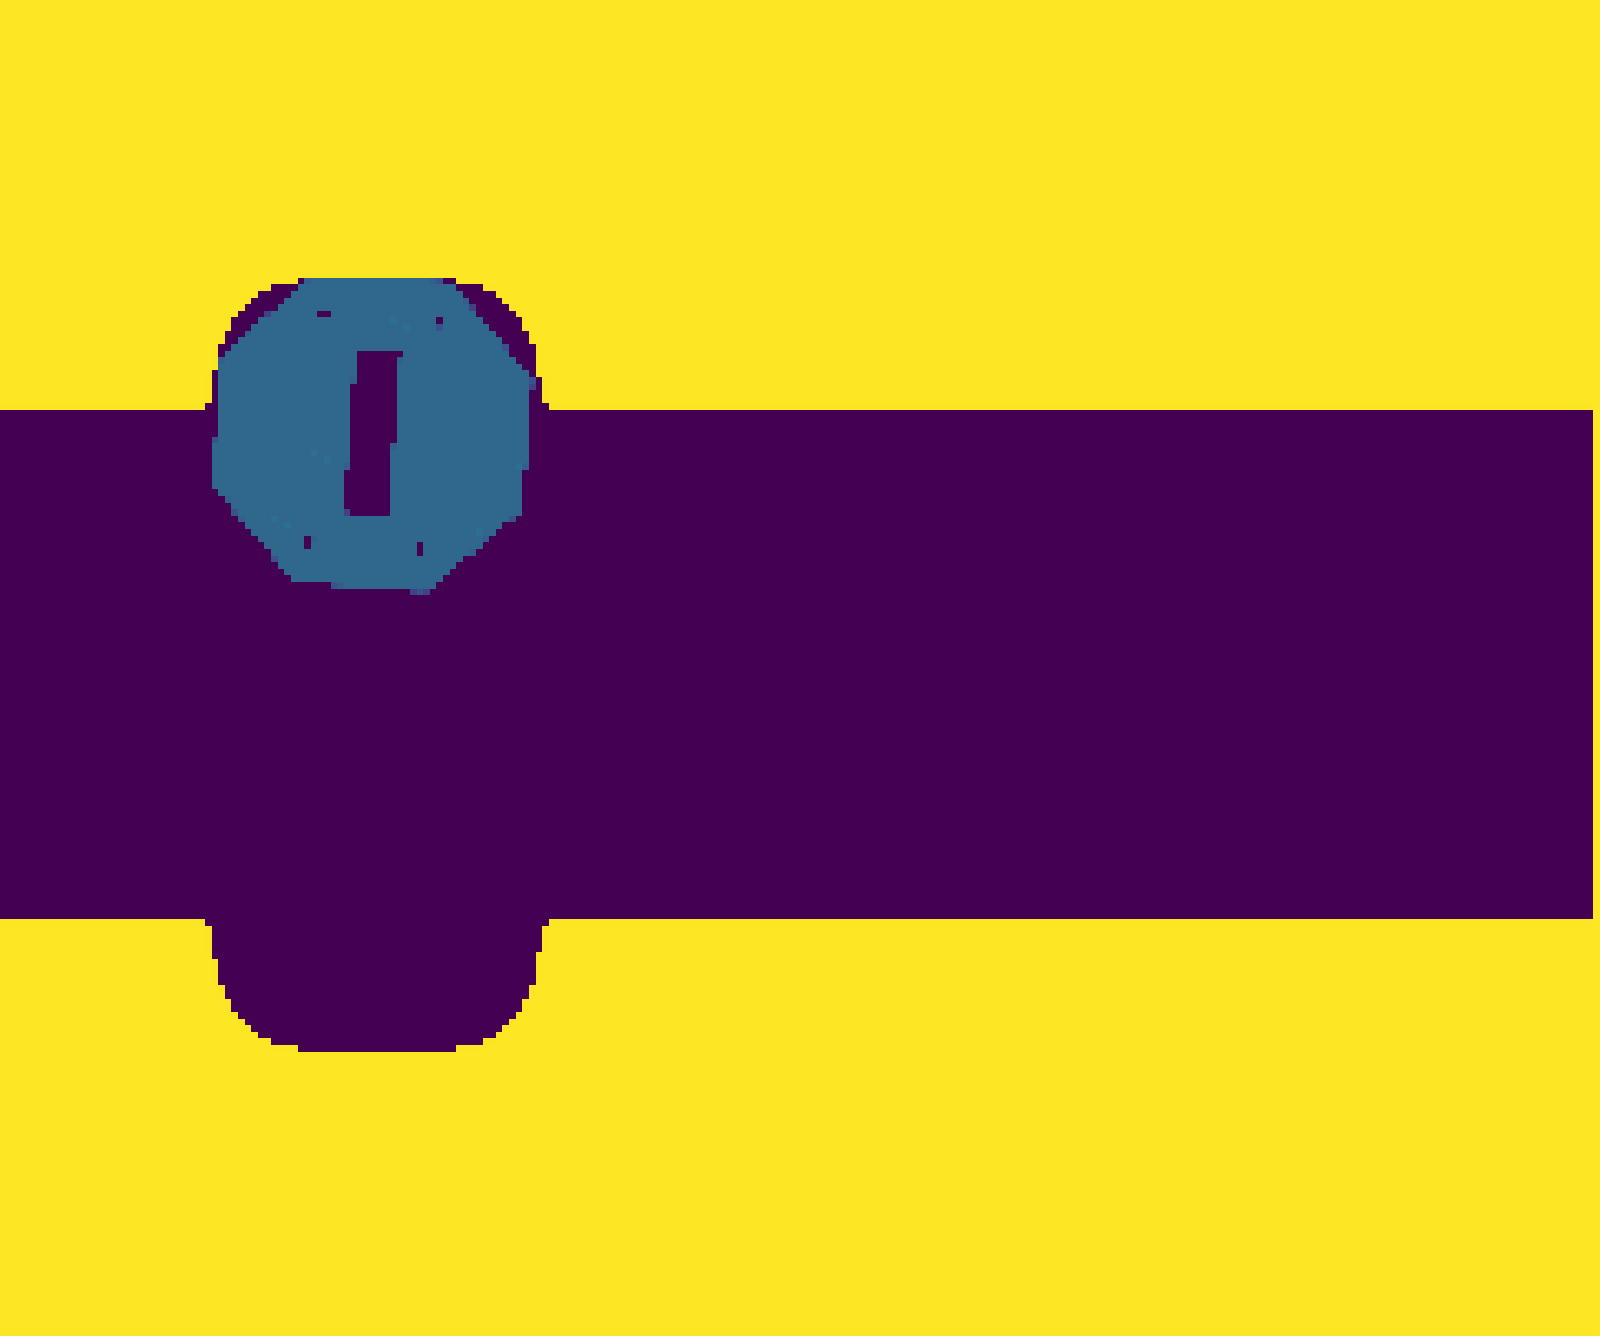
\includegraphics[
            width=\linewidth,
            height=0.20\textheight,
            keepaspectratio
        ]{fig/ch-validation/paralleljaw_IPAIntermediatePlate_NSGA2_100Gen.png}
        \caption{IPA Intermediate Plate; orientation 4}
        \label{fig:qualitative_pj_plate}
    \end{subfigure}\hfill
    \begin{subfigure}[t]{0.48\textwidth}
        \centering
        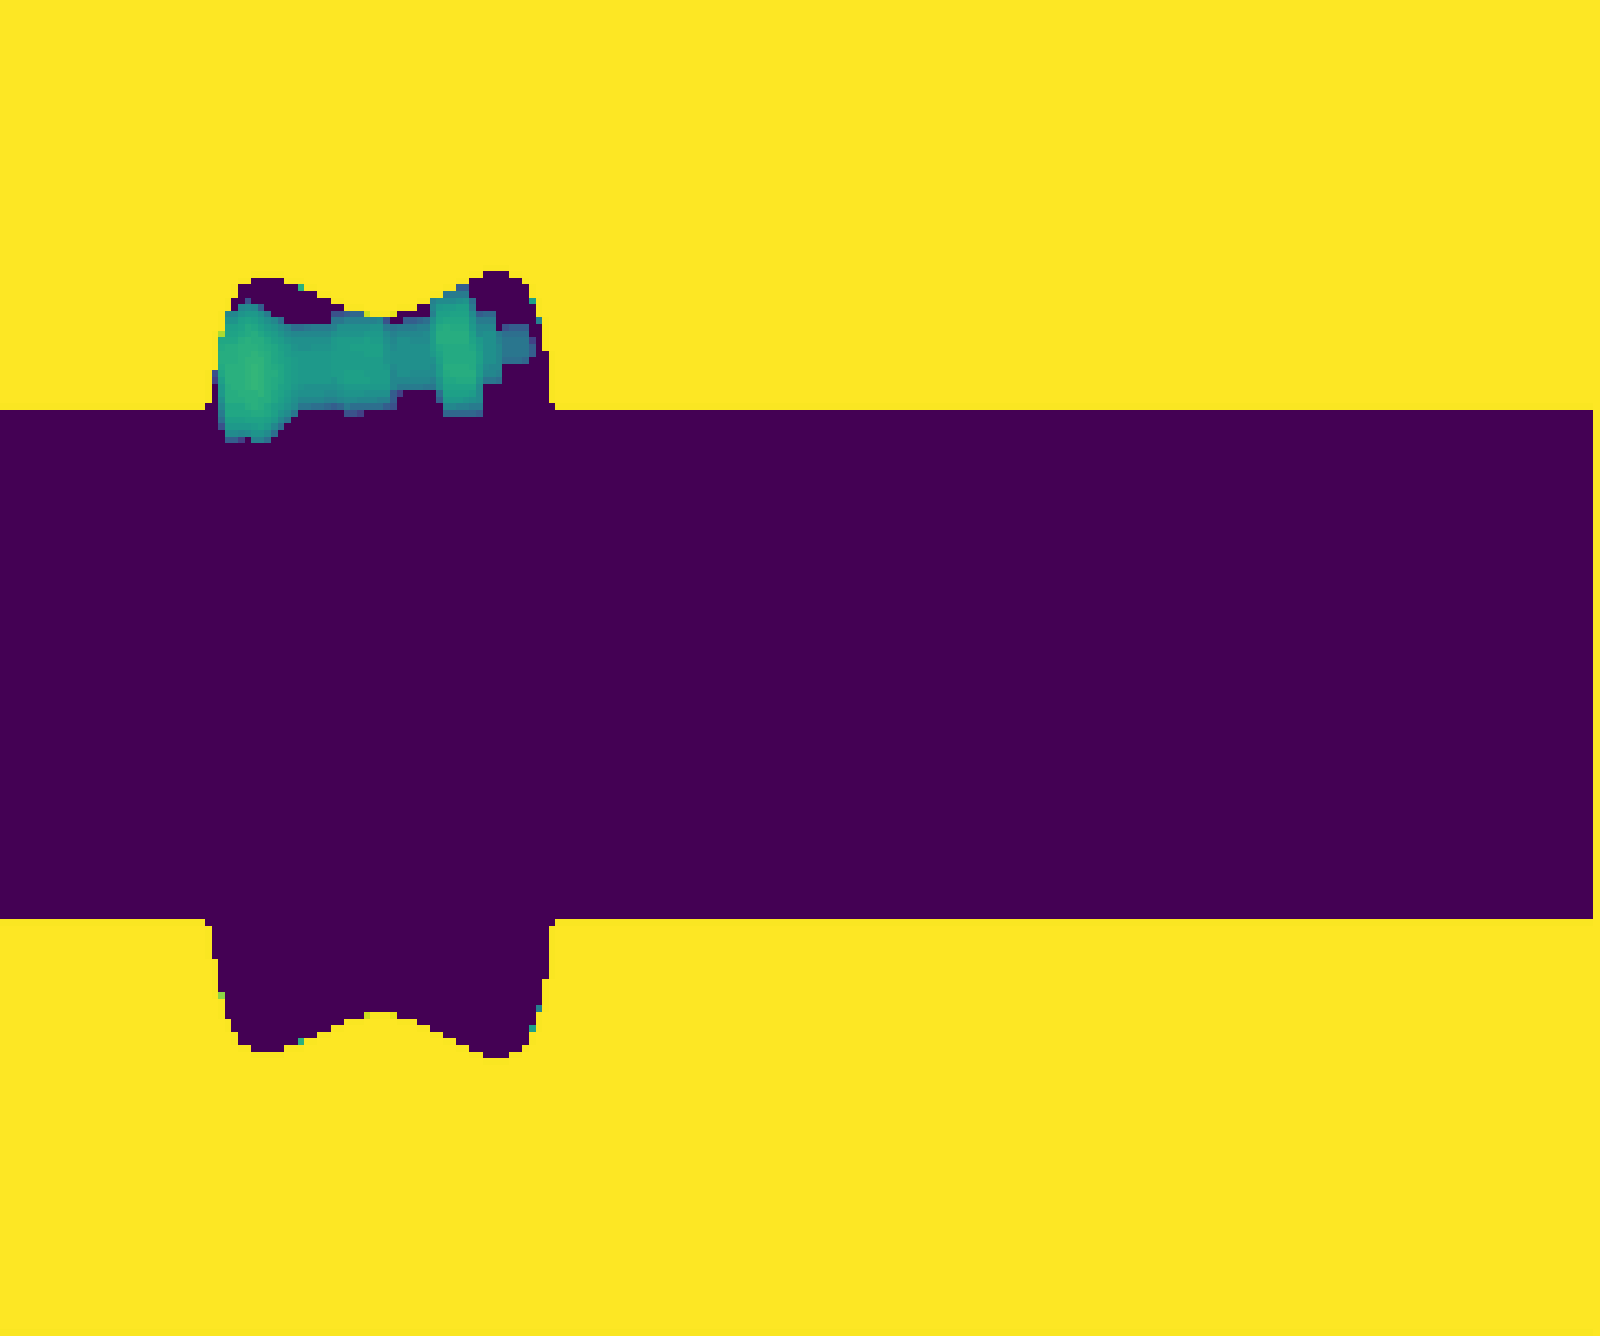
\includegraphics[
            width=\linewidth,
            height=0.20\textheight,
            keepaspectratio
        ]{fig/ch-validation/paralleljaw_MCBA_Knob_NSGA2_100Gen.png}
        \caption{Knob; orientation 4}
        \label{fig:qualitative_pj_knob}
    \end{subfigure}

    \par\medskip

    \begin{subfigure}[t]{0.48\textwidth}
        \centering
        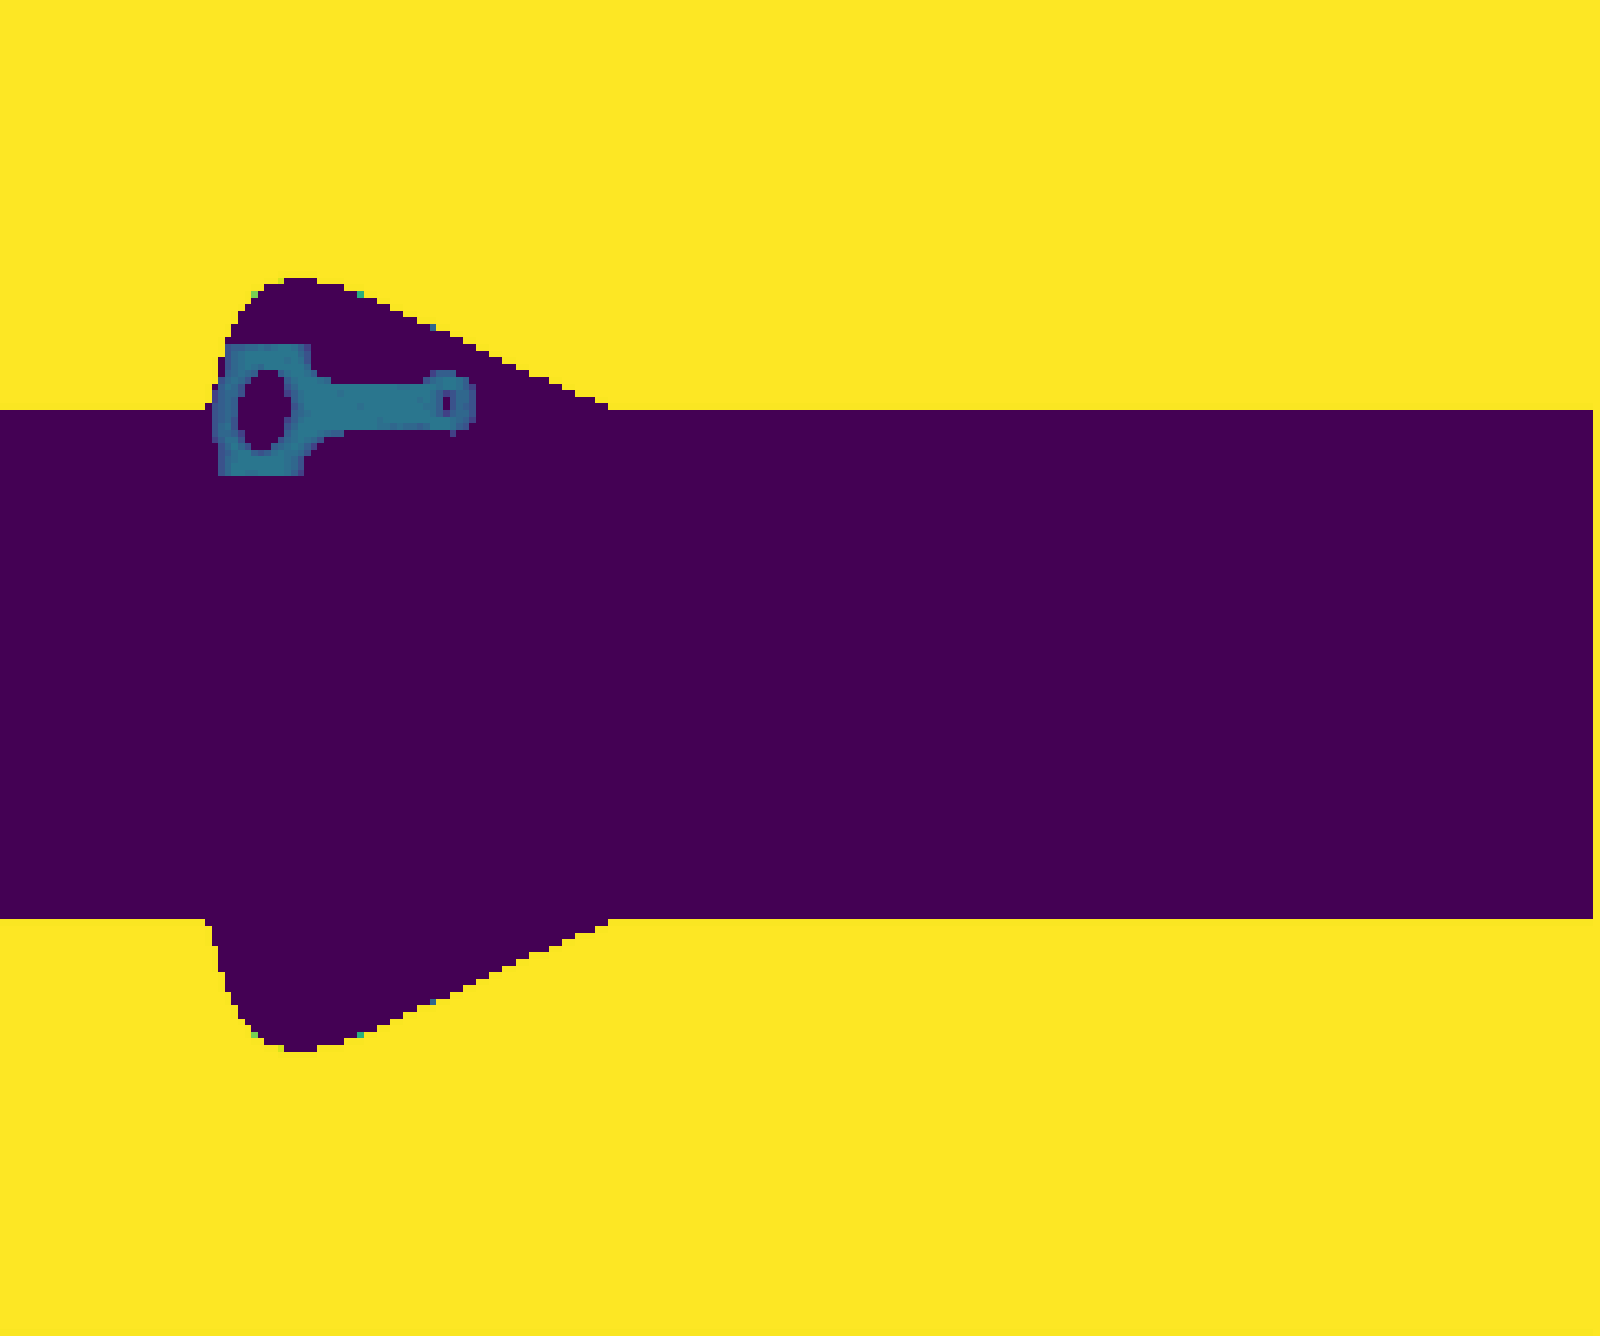
\includegraphics[
            width=\linewidth,
            height=0.20\textheight,
            keepaspectratio
        ]{fig/ch-validation/paralleljaw_IPAConnectingRod_NSGA2_100Gen.png}
        \caption{Connecting rod; orientation 1}
        \label{fig:qualitative_pj_rod}
    \end{subfigure}\hfill
    \begin{subfigure}[t]{0.48\textwidth}
        \centering
        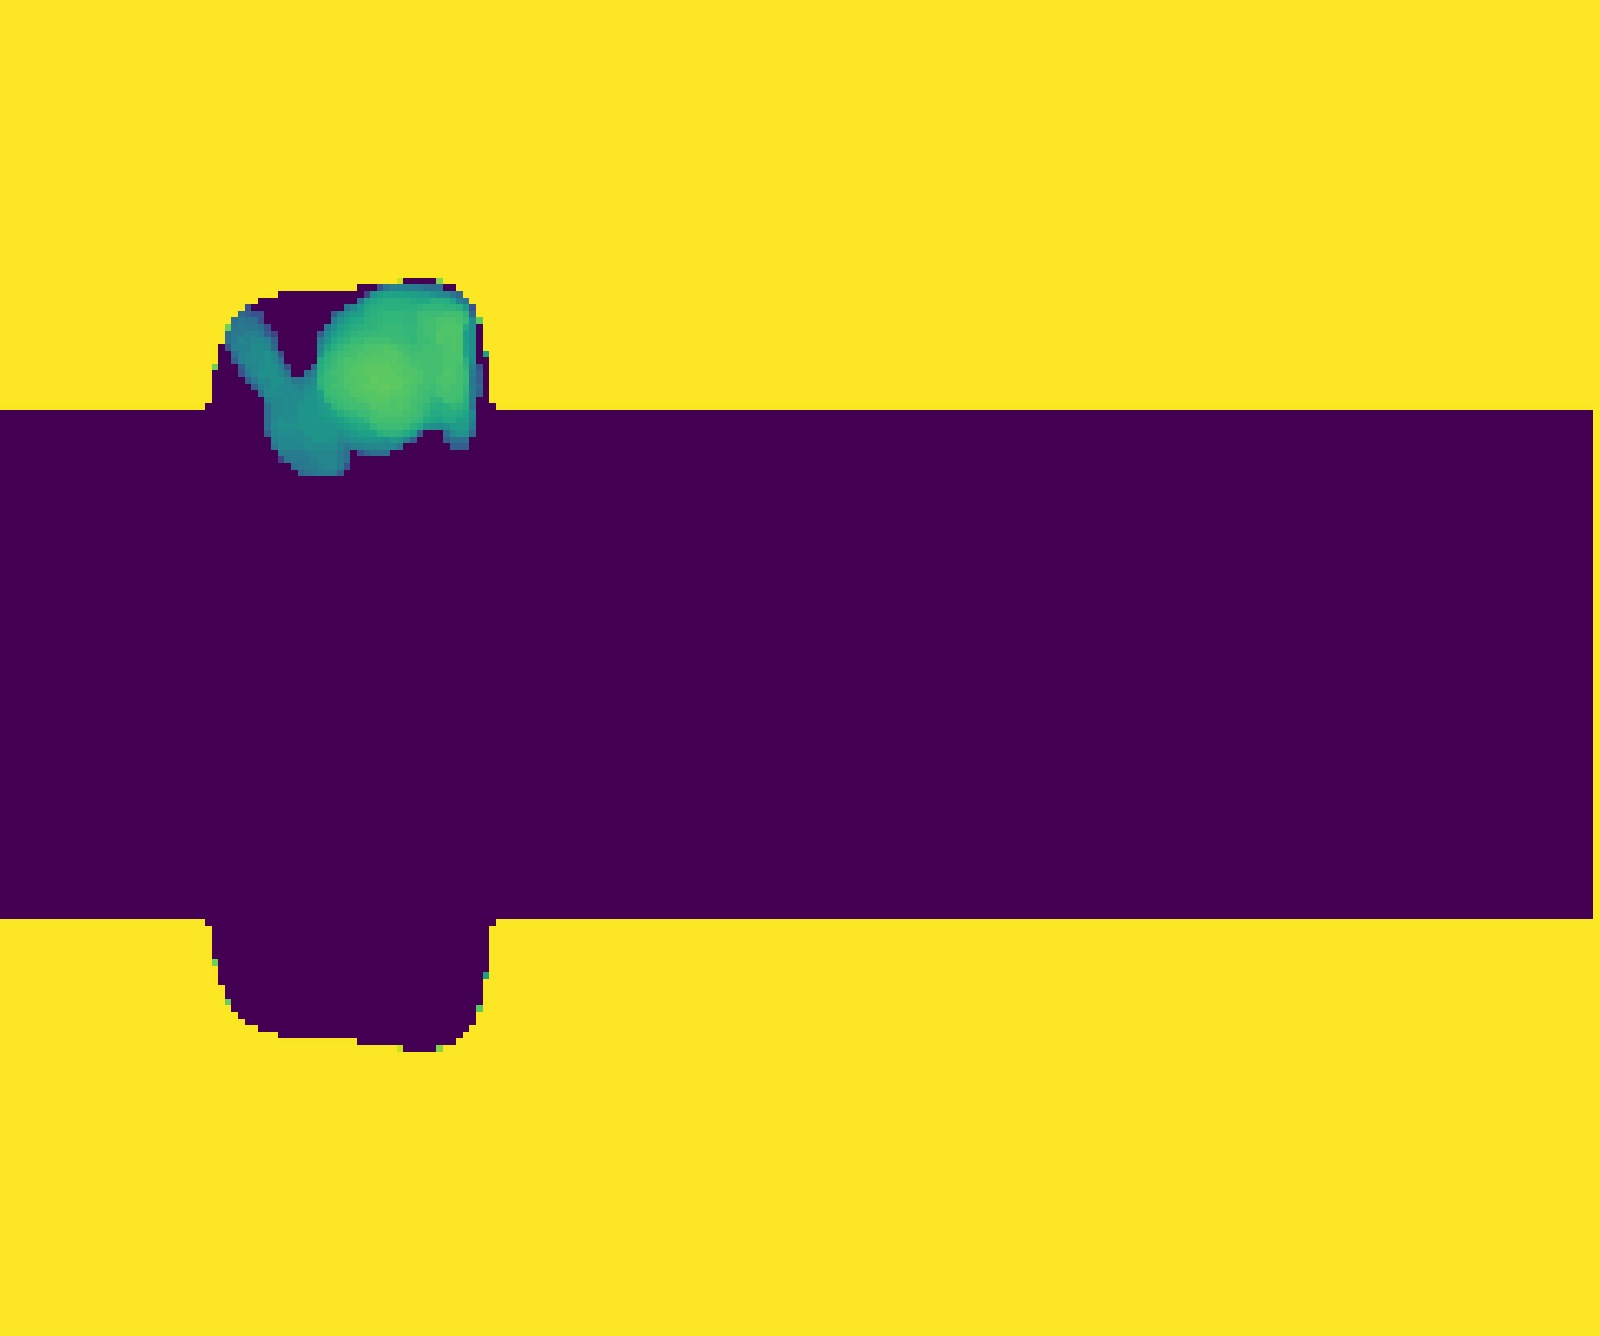
\includegraphics[
            width=\linewidth,
            height=0.20\textheight,
            keepaspectratio
        ]{fig/ch-validation/paralleljaw_IPABunny_NSGA2_100Gen.png}
        \caption{Stanford Bunny; orientation 4}
        \label{fig:qualitative_pj_bunny}
    \end{subfigure}

    \caption{Combined occupancy projections for selected NSGA-II
    parallel-jaw solutions. Each image shows the orientation with the
    highest proximity KPI for the corresponding solution.}
    \label{fig:qualitative_two_finger}
\end{figure}

The decision vector is
$\mathbf{q}_{\mathrm{PJ}}=(\ell_{\mathrm{gn}},h_1,h_2,h_3)$, with all
four parameters in millimeters. The objective vector contains the
proximity KPIs $(k_1,k_2,k_3,k_4)$ in the configured orientation order:

\begin{itemize}
    \item \textbf{IPA Intermediate Plate:}
    $\mathbf{q}_{\mathrm{PJ}}\approx
    (26.4661,\,9.7092,\,9.9724,\,9.7111)$;
    objectives $(0.4605,\,0.2966,\,0.3529,\,0.5735)$.

    \item \textbf{Knob:}
    $\mathbf{q}_{\mathrm{PJ}}\approx
    (27.2187,\,9.6728,\,7.1746,\,9.9716)$;
    objectives $(0.9413,\,0.8044,\,0.7961,\,1.0045)$.

    \item \textbf{Connecting rod:}
    $\mathbf{q}_{\mathrm{PJ}}\approx
    (31.7062,\,9.9189,\,7.1617,\,3.4176)$;
    objectives $(0.4033,\,0.1058,\,0.1187,\,0.1002)$.

    \item \textbf{Stanford Bunny:}
    $\mathbf{q}_{\mathrm{PJ}}\approx
    (22.3557,\,8.7552,\,9.2349,\,9.9188)$;
    objectives $(0.5210,\,0.4857,\,0.7231,\,0.7739)$.
\end{itemize}

The objective vectors show that a contour does not necessarily obtain
the same proximity score in every orientation. For example, the
selected connecting-rod contour has a higher score in orientation 1
than in its other three orientations. The scores are scaled geometric
KPIs and are interpreted within each workpiece problem.

The projections provide a qualitative view of the voxelized
arrangements. They do not distinguish the workpiece from the gripper
in the combined occupancy and do not show both jaws moved to their
selected positions. Each image also shows only the highest-scoring
orientation of the selected solution. The images therefore do not
independently establish contact, collision-free placement, or grasp
stability.

% ============================================================================
\section{Bayesian Optimization Results}
\label{sec:results_bayesian}

Bayesian optimization was carried out in two attempts. The main attempt was
terminated due to its runtime and did not produce any result files.
Subsequently, a minimal test was performed on a single gripper--workpiece pair
to obtain indicative results. This test consists of a single run ($n=1$) and
serves as a starting point for future work rather than as a basis for a
conclusive evaluation. Its limitations are discussed in
Section~\ref{sec:limitations}.
% TODO: check the label of the limitations chapter.

\subsection{Main Attempt}
\label{subsec:results_bayesian_main}

The runs were configured for 100 batches of 10 trials, corresponding to a planned budget
of 1{,}000 evaluations. Four workpiece optimizations ran simultaneously in separate
processes. The runs were stopped manually after more than 90~h; the reported progress was
approximately 450 trials per run. No final result files were produced.

The logs indicate that candidate generation was time-consuming. Batches of ten
trials were marked completed within seconds after their generation, whereas
intervals containing Ax and BoTorch warnings lasted substantially longer. This
suggests that model fitting and acquisition optimization contributed to the
runtime, although the logs do not provide separate timings for these steps.

Several factors may have contributed to this cost. For four decision variables
and a batch of ten candidates, joint acquisition optimization would involve $10
\times 4 = 40$ candidate coordinates. In addition, as observations accumulate,
fitting a Gaussian process becomes more expensive
(Section~\ref{subsec:bayesian_moo}). The four processes maintained separate
models and search spaces, but competition for shared computational resources may
also have increased runtime.

The logs further report numerical and optimization warnings:

\begin{itemize}
    \item Repeated \texttt{A not p.d., added jitter of 1.0e-08} warnings show
    that diagonal jitter was added during matrix factorization. Such warnings
    can arise from numerical ill-conditioning, although their cause cannot be
    established from the logs alone.
    \item A \texttt{gen\_candidates\_scipy} optimization reported status
    \texttt{ABNORMAL} and was retried with new initial conditions. Such retries
    can add to candidate-generation time.
    \item Ax reported a \texttt{MultiObjective} without objective thresholds and
    consequently winsorized each objective separately. The effect of this
    configuration on acquisition optimization and runtime was not measured.
\end{itemize}

The runs were therefore interrupted because of the time required, rather than an
unrecoverable exception. Since the logs from concurrent processes are
interleaved and do not isolate model-fitting, acquisition, and evaluation times,
the relative contribution of each factor remains unresolved.

\subsection{Minimal Test on the Connecting Rod}
\label{subsec:results_bayesian_minimal}

After the main attempt was stopped, a minimal test was run for the two-finger gripper on
the Connecting rod only. It used a batch size of 5 and 100 batches, i.e.\ up to 500
evaluations, and was run once ($n=1$). A total of 496 evaluations were completed. The
problem, reference point, and archive-HV definition are the same as for the evolutionary
algorithms in Section~\ref{sec:results_tf}. Only the archive HV and the runtime are
reported. No standard deviation is available because $n=1$.

Table~\ref{tab:pj_bayesian_connecting_rod} adds the Bayesian run to the two-finger results
on the Connecting rod. After 496 evaluations, the Bayesian run reaches an archive HV of
0.0281. This is about 87\,\% of the highest final HV (NSGA-II, 0.0323) and about 91\,\% of
that of CMOPSO (0.0309). It is about 9\,\% higher than the final HV of MOEA/D (0.0259).
The evolutionary algorithms used 10{,}000 evaluations, about 20 times more.

\begin{table}[htbp]
    \centering
    \caption{Two-finger results on the Connecting rod, including the Bayesian minimal test.
    Evolutionary algorithms: $n=3$ runs, 10{,}000 evaluations. Bayesian: $n=1$ run,
    496 evaluations, no standard deviation available for Bayesian.}
    \label{tab:pj_bayesian_connecting_rod}
    \begin{tabular}{@{}lccc@{}}
        \toprule
        \textbf{Algorithm} & \textbf{Archive HV} $\uparrow$ & \textbf{Runtime (s)} & \textbf{Time per eval.\ (s)} \\
        \midrule
        CMOPSO    & $0.0309 \pm 0.0003$ & $27849.4 \pm 1.7$ & 2.8 \\
        MOEA/D    & $0.0259 \pm 0.0003$ & $72605.3 \pm 14.3$ & 7.3 \\
        NSGA-II   & {\boldmath$0.0323 \pm 0.0003$} & $46526.8 \pm 14061.9$ & 4.7 \\
        NSGA-III  & $0.0318 \pm 0.0008$ & $38407.6 \pm 24954.0$ & 3.8 \\
        SMS-EMOA  & $0.0320 \pm 0.0003$ & $30505.6 \pm 7.9$ & 3.1 \\
        \midrule
        Bayesian ($n=1$) & $0.0281$ & $66684.3$ & 134.4 \\
        \bottomrule
    \end{tabular}
\end{table}

\begin{figure}[H]
    \centering
    \figslot{fig/ch-result/PJ_Bayesian_hv_progression.png}
    \caption{Cumulative archive hypervolume over evaluations on the Connecting rod
    (two-finger gripper). Evolutionary algorithms: mean across $n=3$ runs, shading
    $\pm 1$ sample SD. Bayesian: single run of 496 evaluations, no shading.}
    \label{fig:bayesian_hv_progression}
\end{figure}

Figure~\ref{fig:bayesian_hv_progression} shows that the Bayesian curve rises much faster
per evaluation than those of all evolutionary algorithms. It reaches an HV of about 0.026
within the first 100--150 evaluations, where the evolutionary algorithms are at about
0.014--0.017. The curve then increases slowly and ends at about 0.028 after 496
evaluations. At equal numbers of evaluations, the Bayesian run is therefore above all
evolutionary algorithms. CMOPSO, NSGA-II, NSGA-III, and SMS-EMOA exceed this value only
after about 1{,}800 to 3{,}000 evaluations, and MOEA/D does not reach it within 10{,}000
evaluations.


The runtime of the test was 66{,}684~s (about 18.5~h), or about 134~s per evaluation. The
evolutionary algorithms needed about 2.8 to 7.3~s per evaluation, so the Bayesian run
is roughly 18 to 48 times more expensive per evaluation. The runs were carried out on different
GPUs, so the measured times are not directly comparable. The runtimes are therefore
indicative only and are not a conclusive result.
